\section{Aufbau und Durchführung des Versuchs}
\subsection{Messaufbau}
Der Aufbau der Messapparatur ist in Abbildung \ref{fig:aufbau} dargestellt.
\begin{figure}[!ht]
	\centering
	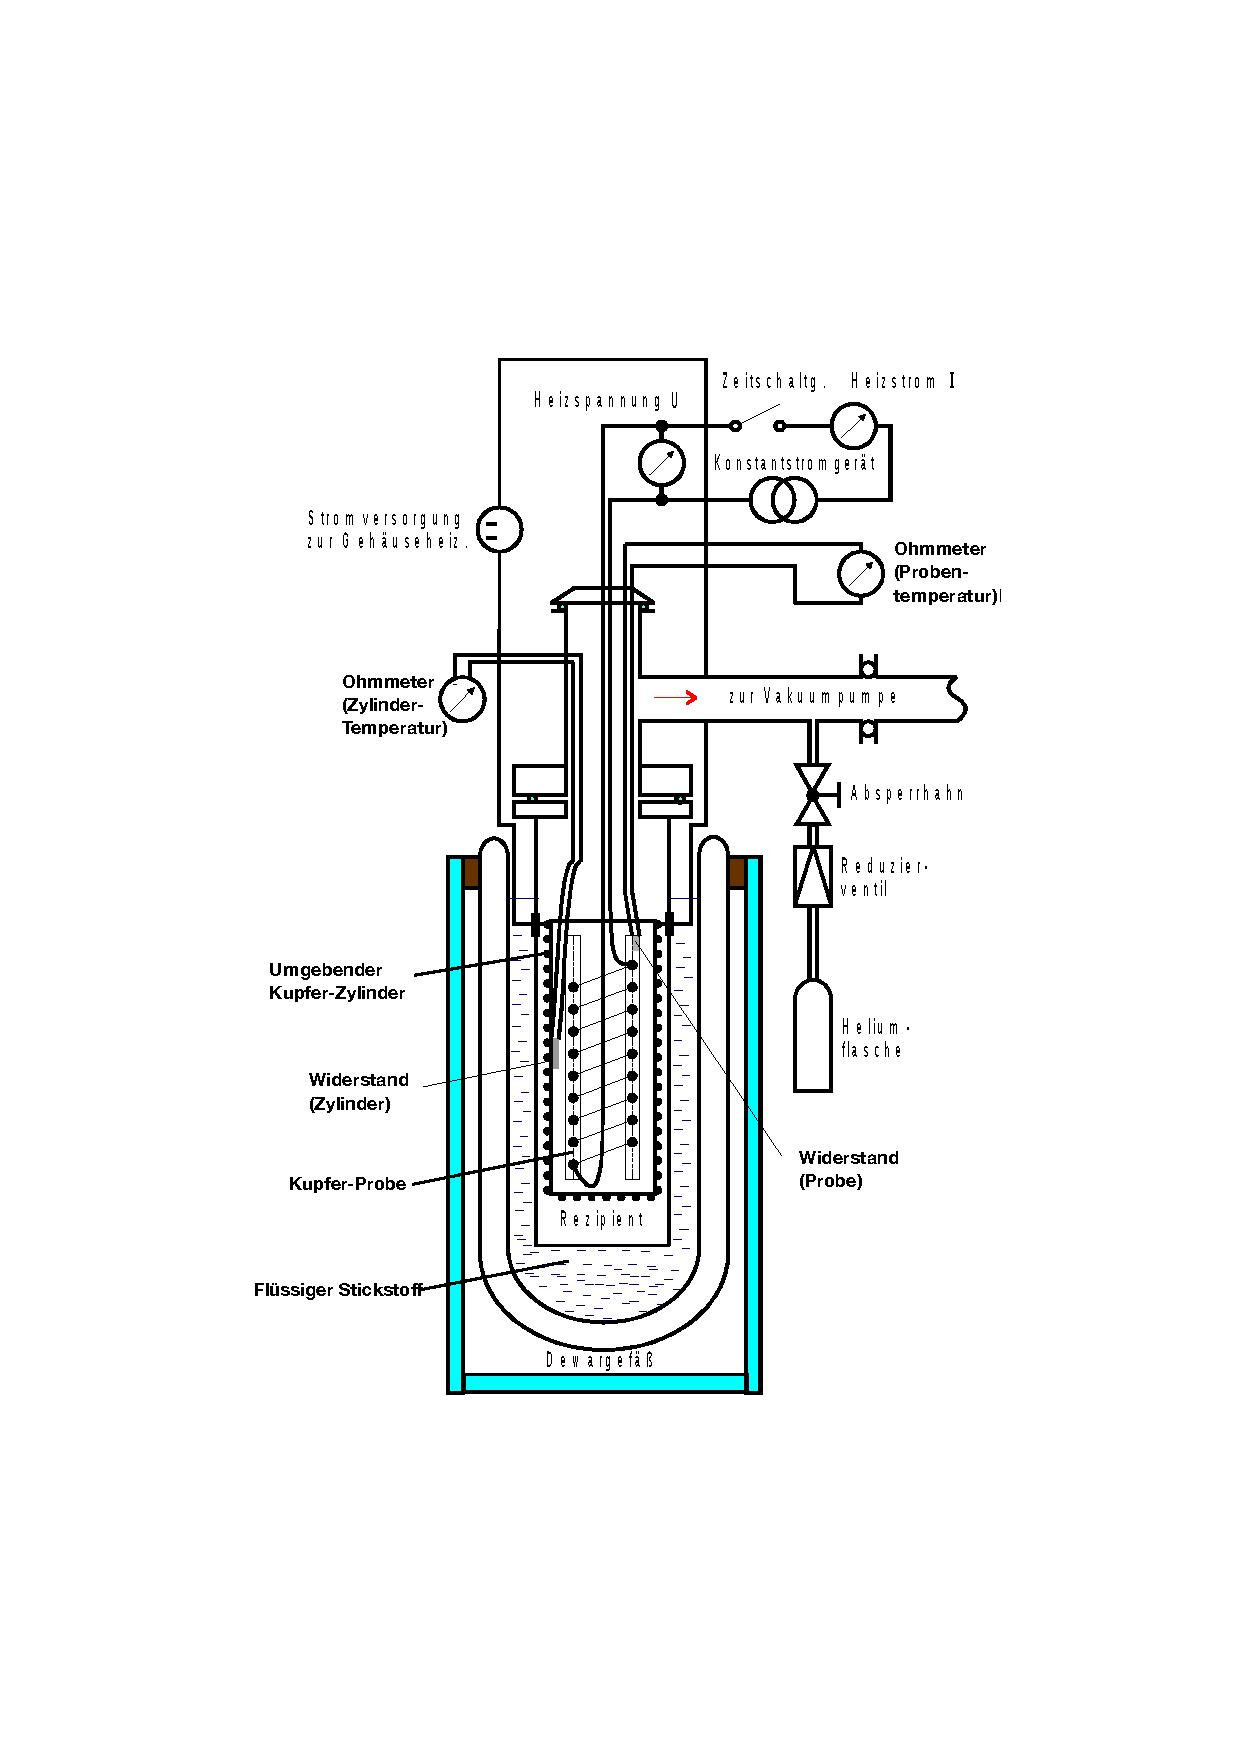
\includegraphics[width=0.7\textwidth]{content/images/aufbau.pdf}
    \caption{Skizze des Versuchsaufbaus \cite{anleitung}, modifiziert.}
    \label{fig:aufbau}
\end{figure}
Der Aufbau befindet sich zur thermischen Isolation in einem Dewargefäß.
Das Dewargefäß wird mit flüssigem Stickstoff gefüllt, um den darin Rezipienten zu kühlen, der darin liegt.
Ein Rezipient ist eine evakierbare Kammer.
Dieser ist mit einer Vakuumpumpe und mit einer Helium-Flasche verbunden.
Im Rezipienten befindet sich ein Kupferzylinder, in dem sich wiederum die stabförmige Kupferprobe befindet.
Beide Teile (Zylinder und Probe) sind mit je einer Heizspule umwickelt und können separat mit einem jeweiligen Heizstrom beheizt werden.
Außen am Zylinder und zwischen Zylinder und Probe sind Pt-100-Messwiderstände angebracht.
Diese Bezeichnung spezifiziert einen temperaturabhängigen Widerstand, der bei $\SI{0}{K}$ einen Widerstand von $R = \SI{100}{\ohm}$ hat.
Diese werden über angeschlossene Ohmmeter ausgelesen.
Später wird aus dem Widerstand die in der Probe deponierte Energie berechnet.


Der Rezipient wird mit Helium gefüllt, um einerseits bei den verwendeten Temperaturen eine beständige Gasphase im Rezipienten zu gewährleisten.
Durch die Arbeit mit flüssigem Stickstoff besteht bei einem Rezipienten voller Luft die Gefahr, dass der Luftsauerstoff hier kondensiert.
Andererseits wird durch die Verwendung von Helium eine Vereisung des Kondensationswassers der Luft verhindert.


Die Energie, die der Kupferprobe zugeführt wird, soll vollständig zur Erwärmung dieser genutzt werden.
Die Verluste durch Konvektion, Wärmestrahlung und Wärmeleitung werden durch verschiedene Komponenten des Aufbaus weitestgehend unterbunden.
Konvektion wird durch das Evakuieren des Rezipienten verhindert.
Der Energieverlust durch Wärmestrahlung wird durch den die Probe umgebenden Kupferzylinder minimiert.
Da beide Teile aus dem gleichen Material bestehen, strahlen sie bei gleicher Temperatur im gleichen Maße Wärme ab.
So wird ein möglicher Energieverlust der Probe durch Wärmestrahlung durch eine gleich große eingehende Wärmestrahlung vom Kupferzylinder ausgeglichen.
Mit diesem Setting ist auch der Energieverlust durch Wärmeleitung beseitigt.
Kupferprobe und -zylinder grenzen aneinander und werden mit den Heizspulen auf der gleichen Temperatur gehalten.
Bei einem verschwindenden Temperaturgradienten verschwindet auch die Wärmeleitung im Material.

\subsection{Vorgehen und Durchführung des Versuch}
\paragraph{Vorbereitung}
Zunächst wird der Rezipient evakuiert.
Anschließend wird der Rezipient mit Helium geflutet.
Das Dewargefäß wird so weit wie möglich mit flüssigem Stickstoff bei ca. $\SI{80}{K}$ gefüllt.
Die Ohmmeter für den Widerstand am Zylinder und an der Probe werden gestartet.
Nun wird gewartet, bis die Widerstände der Probe und des Kupferzylinders im Gleichgewicht sind, was eine angeglichene Temperatur der beiden Bauteile bedeutet.
Zwischendurch wird der flüssige Stickstoff nachgefüllt.
Sobald die Probe und der Zylinder einen gleichmäßigen Widerstand von $R \approx \SI{20}{\ohm}$ haben, wird der Rezipient evakuiert.
Nach einer weiteren kurzen Wartezeit werden die Heizströme und die Heizspannungen eingeschaltet.

\paragraph{Durchführung der Messung}
Die Messung funktioniert über das kontinuierliche Aufwärmen der Kupferelemente.
Durch die Temperaturänderung ändert sich der Widerstand der PT-100-Widerstände, und die deponierte Energie im Material kann gemessen werden.
Als Messdaten werden die Messdauer $t$, der Widerstandswert an der Probe $R_{\text{i}}$, der Widerstandswert an dem Zylinder $R_{\text{a}}$, die Heizspannung $U_{\text{i}}$ und der Heizstrom $I_{\text{i}}$ der Probe und Heizstrom des Zylinders $I_{\text{a}}$ aufgenommen.
Während der Messung werden die Heizspannung $U_{\text{i}}$ und der Heizstrom $I_{\text{i}}$ der Heizspule an der Probe nicht aktiv erhöht.
Lediglich mit dem Heizstrom des Zylinders wird auf die Erwärmung des Aufbaus reagiert.
Weist die Probe einen größeren Widerstandswert auf als der Zylinder, so wird der Zylinder verstärkt geheizt.
Weist der Zylinder einen größeren Widerstandswert auf, so wird die Heizung des Zylinders gedrosselt.
Die Messdaten werden bis zur Probentemperatur von $T \approx \SI{-50}{°C}$ alle $2\!:\!30 \, \symup{min}$ notiert.
Danach wird bis zum Erreichen der Raumtemperatur alle $\SI{5}{min}$ gemessen.
